El proceso de enumeración trataremos de recabar información de recurso accesibles del sistema 
o aplicación. Para este proceso existen númerosas utilidades, entre las más utilizadas estarían:

En índice de vulnerabilidades web OWASP Top 10, \href{https://wiki.owasp.org/images/5/5e/OWASP-Top-10-2017-es.pdf}{versión 2017}, 
clasifica los vulnerabilidades más comunes encontradas en los datos de aportados por cientos de organizaciones 
y más de 100.000 aplicaciones y servicios web del mundo real.

En su última versión las vulnerabilidades más comunes encontradas fueron las siguientes:

\begin{figure}[h!]  
    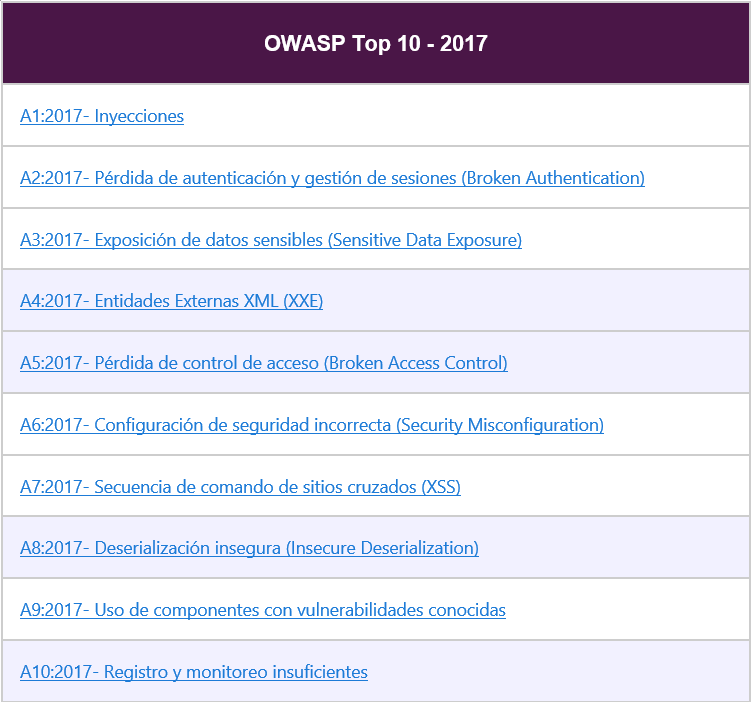
\includegraphics[width=\linewidth]{./imagenes/012_OWASP_Top_10_2017.png}
    \caption{OWASP Top 10 2017.}  
    \label{fig:OWASP Top 10 2017}
\end{figure}

A continuación, detallamos en que consisten cada una de las vulnerabilidades listadas en el OWASP top 10:

\subsection{A1:2017 - Inyecciones}

Las fallas de inyección, como SQL, NoSQL, comandos o LDAP ocurren cuando se envían datos no
confiables a un intérprete, como parte de un comando o consulta. Los datos dañinos del atacante
pueden engañar al intérprete para que ejecute comandos involuntarios o acceda a los datos sin
la debida autorización.

La inyección de SQL (SQLi) es uno de los tipos de ataques de inyección de código más
comunes y peligrosos, aprovechados por los atacantes con la intención de obtener
información no autorizada o en sí generar problemas en los servidores de base de datos y
comportamiento de aplicaciones.

Por Ejemplo, en la siguiente aplicación tenemos un formulario para mostrar 
la información de un usuario a partir de su identificador (ID):

\begin{figure}[h!]  
    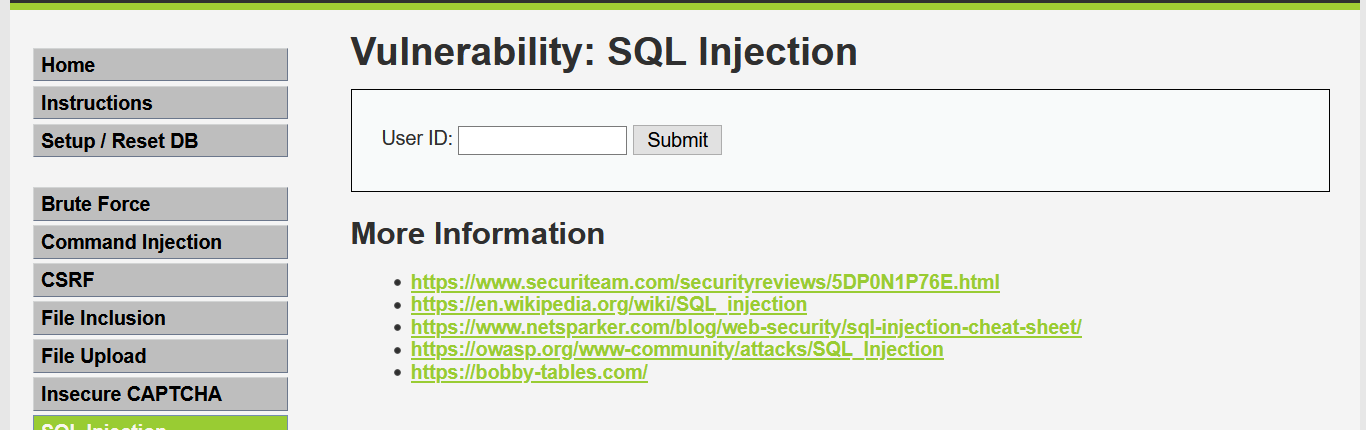
\includegraphics[width=\linewidth]{./imagenes/013_SQLi_Example_1.png}
    \caption{Aplicación vulnerable SQLi.}  
    \label{fig:SQLi 1}
\end{figure}

Un uso normal generaría este tipo de peticiones:

\begin{figure}[h!]  
    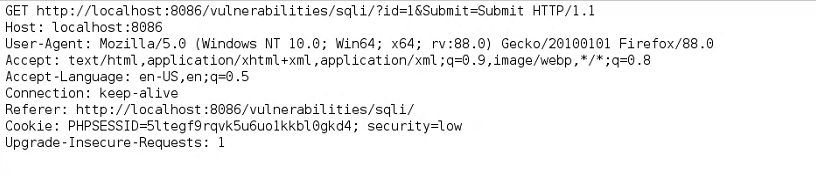
\includegraphics[width=\linewidth]{./imagenes/013_SQLi_Example_2.png}
    \caption{Petición normal.}  
    \label{fig:SQLi 2}
\end{figure}

\begin{verbatim}
    %' union select user,password from users# 
\end{verbatim}

Se genera la siguiente petición:

\begin{figure}[h!]  
    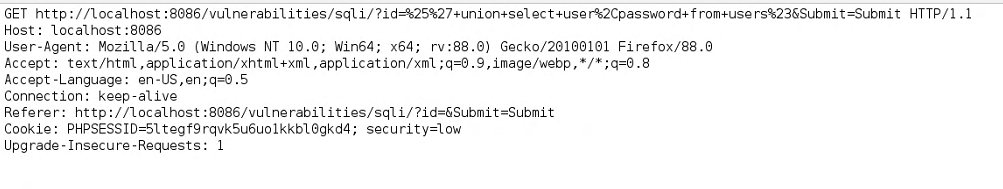
\includegraphics[width=\linewidth]{./imagenes/013_SQLi_Example_3.png}
    \caption{SQLi example.}  
    \label{fig:SQLi 3}
\end{figure}

El resultado será que la aplicación nos devuelve todos los usuarios y password almacenados en la Base de datos:

\begin{figure}[h!]  
    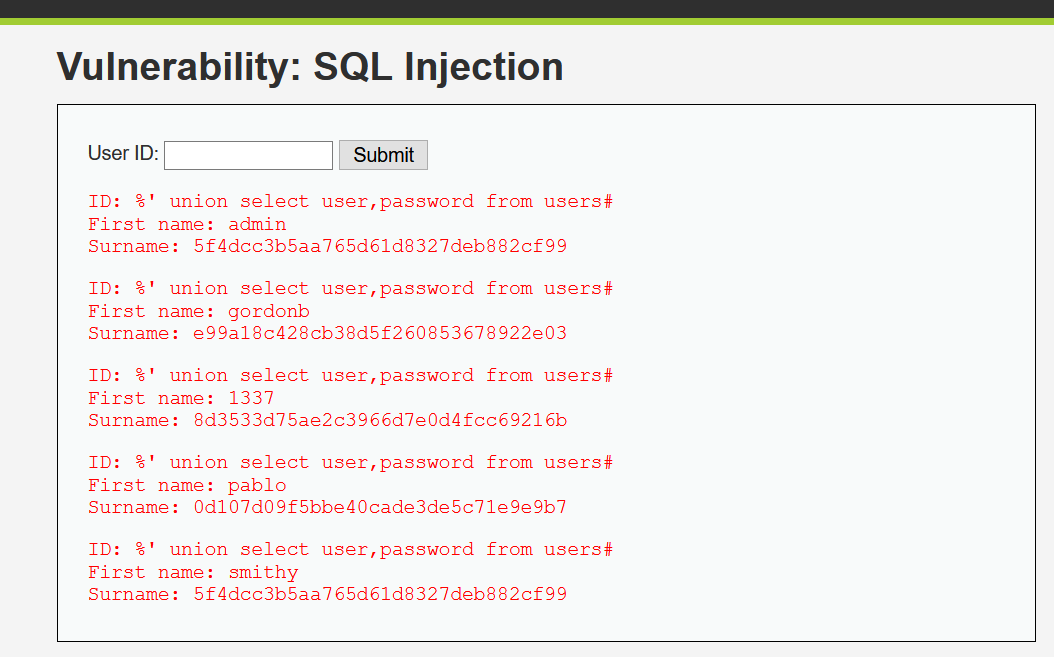
\includegraphics[width=\linewidth]{./imagenes/013_SQLi_Example_4.png}
    \caption{Resultado ataque SQLi.}  
    \label{fig:SQLi 3}
\end{figure}

\subsection{A2:2017 - Pérdida de autenticación y gestión de sesiones (Broken Authentication)}

Las funciones de la aplicación relacionadas a autenticación y gestión de sesiones son
implementadas incorrectamente, permitiendo a los atacantes comprometer usuarios y
contraseñas, token de sesiones, o explotar otras fallas de implementación para asumir la
identidad de otros usuarios (temporal o permanentemente).

En los últimos años se han detectado numerosas aplicaciones, sobre todo la que hacen uso de api para 
la gestión de los datos, que hacen uso de JSON Web Tokens (JWT) para la autenticación y autorización. 

\begin{figure}[h!]  
    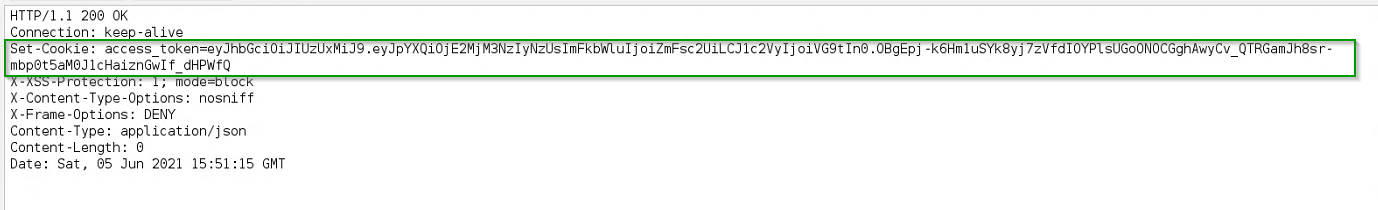
\includegraphics[width=\linewidth]{./imagenes/014_BrokenAuthentication_1.png}
    \caption{Token JWT.}  
    \label{fig:Token JWT}
\end{figure}

La captura de este token permite a los atacantes a realizar peticiones en nombre del usuario, puesto que, 
si decodificamos el token, podemos ver que identifica a un usuario concreto

\begin{figure}[h!]  
    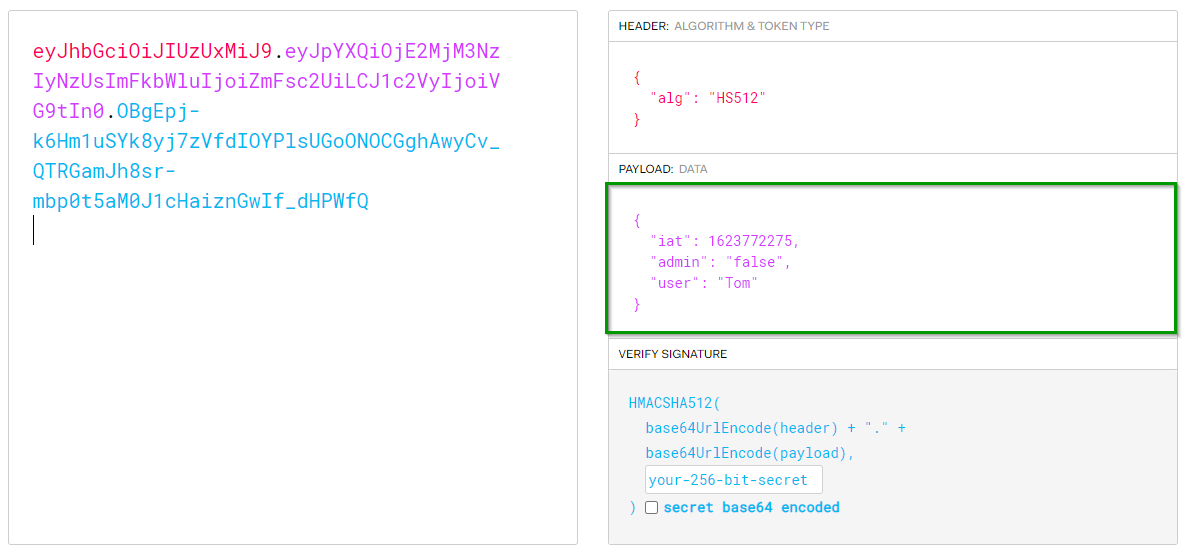
\includegraphics[width=\linewidth]{./imagenes/014_BrokenAuthentication_2.png}
    \caption{Token JWT decodificado.}  
    \label{fig:Token JWT decodificado}
\end{figure}

Lo cual nos permite realizar cualquier petición en nombre del usuario haciendo uso de su token JWT.

\begin{figure}[h!]  
    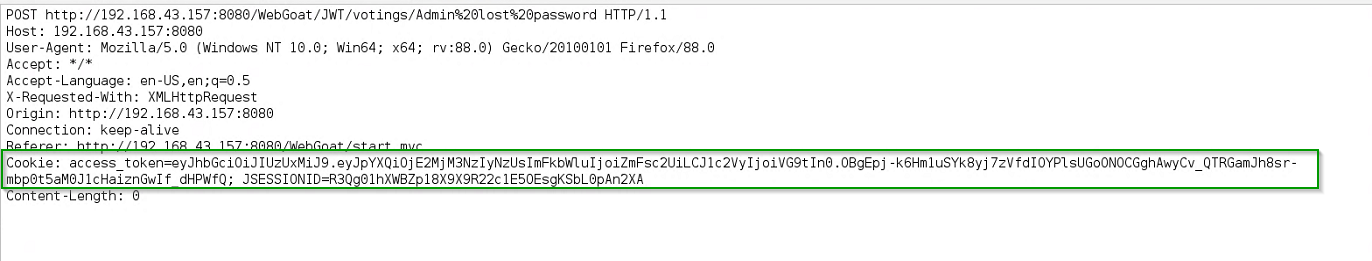
\includegraphics[width=\linewidth]{./imagenes/014_BrokenAuthentication_3.png}
    \caption{Token JWT decodificado.}  
    \label{fig:Broken Authentication attack}
\end{figure}

\subsection{A3:2017 - Exposición de datos sensibles (Sensitive Data Exposure)}

Muchas aplicaciones y servicios web no protegen adecuadamente datos sensibles, tales como
información financiera, de salud o Información Personalmente Identificable (PII). Los atacantes
pueden robar o modificar estos datos protegidos inadecuadamente para llevar a cabo fraudes
con tarjetas de crédito, robos de identidad u otros delitos. Los datos sensibles requieren métodos
de protección adicionales, como el cifrado en almacenamiento y tránsito. 

\subsection{A4:2017 - XML External Entities (XXE)}

Muchos procesadores XML antiguos o mal configurados evalúan referencias a entidades externas en 
documentos XML. Las entidades externas pueden utilizarse para revelar archivos internos mediante la URI 
o archivos internos en servidores no actualizados, escanear puertos de la LAN, ejecutar código de forma
 remota y realizar ataques de denegación de servicio (DoS).

Una entidad XML permite definir etiquetas que serán reemplazadas por contenido cuando se analice 
el documento XML. En general, existen tres tipos de entidades: 

\begin{itemize}
    \item Entidades internas.
    \item Entidades externas.
    \item Entidades parametrizadas.
\end{itemize}

Una entidad debe ser definida en el “Document Type Definition” (DTD), vemos un ejemplo:

\begin{listing}[h]
    \inputminted{xml}{./Ficheros/DTD_example.xml}
    \caption{DTD example}
    \label{listing:1}
\end{listing}

En este caso el parser de XML carga la entidad externa \textbf{"SYSTEM"} que obtendrá el contenido del 
fichero \textbf{"/etc/passwd"} y devolverá el contenido de este fichero en la respuesta:

\begin{figure}[h!]  
    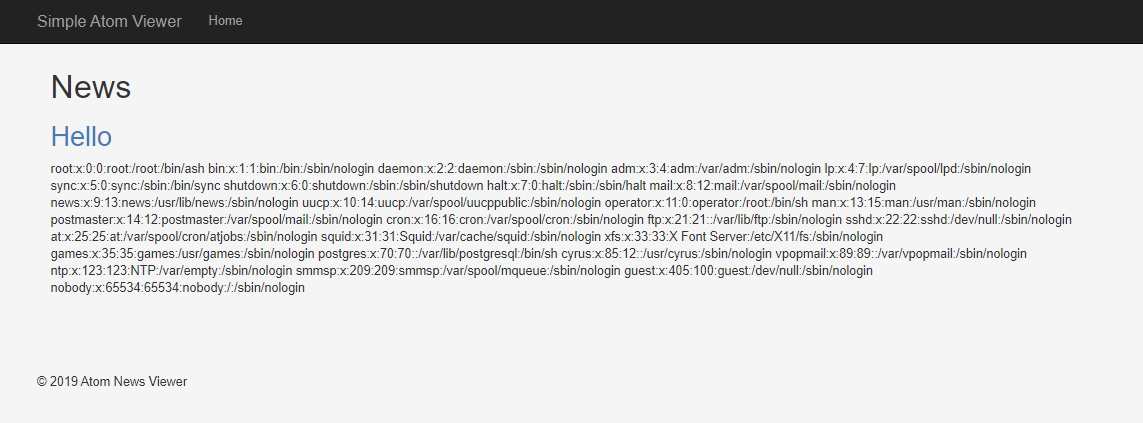
\includegraphics[width=\linewidth]{./imagenes/015_XXE_Attack_1.png}
    \caption{Ataque XXE.}  
    \label{fig:XXE attack}
\end{figure}

Por lo tanto, un ataque de entidad externa XML es un tipo de ataque contra una aplicación que analiza 
la entrada XML. Este ataque ocurre cuando la entrada XML que contiene una referencia a una 
entidad externa es procesada por un analizador XML configurado débilmente. 

Este ataque puede conducir a la divulgación de datos confidenciales, denegación de servicio, falsificación 
de solicitudes del lado del servidor, escaneo de puertos desde la perspectiva de la máquina donde se 
encuentra el analizador y otros impactos del sistema.

\subsection{A5:2017 - Pérdida de control de acceso (Broken Access Control)}

Las restricciones sobre lo que los usuarios autenticados pueden hacer no se aplican
correctamente. Los atacantes pueden explotar estos defectos para acceder, de forma no
autorizada, a funcionalidades y/o datos, cuentas de otros usuarios, ver archivos sensibles,
modificar datos, cambiar derechos de acceso y permisos, etc. 

\subsection{A6:2017 - Configuración de seguridad incorrecta (Security Misconfiguration)}

La configuración de seguridad incorrecta es un problema muy común y se debe en parte a
establecer la configuración de forma manual, ad hoc o por omisión (o directamente por la falta de
configuración). 

Son ejemplos: S3 buckets abiertos, cabeceras HTTP mal configuradas, mensajes
de error con contenido sensible, falta de parches y actualizaciones, frameworks, dependencias y
componentes desactualizados, etc.

\subsection{A7:2017 - Secuencia de comando de sitios cruzados (XSS)}

Los XSS ocurren cuando una aplicación toma datos no confiables y los envía al navegador web
sin una validación y codificación apropiada; o actualiza una página web existente con datos
suministrados por el usuario utilizando una API que ejecuta JavaScript en el navegador. Permiten
ejecutar comandos en el navegador de la víctima y el atacante puede secuestrar una sesión,
modificar (defacement) los sitios web, o redireccionar al usuario hacia un sitio malicioso.

Por ejemplo, si tenemos una aplicación como la siguiente con un formulario de entrada de datos como el siguiente:

\begin{figure}[h!]  
    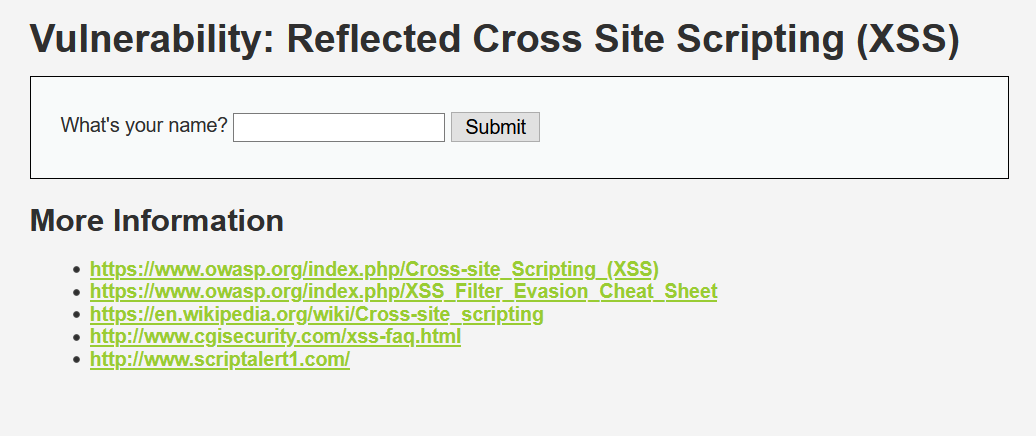
\includegraphics[width=\linewidth]{./imagenes/016_XSS_1.png}
    \caption{Aplicacion insegura XXS.}  
    \label{fig:Aplicacion insegura XXS.}
\end{figure}

Si introducimos el siguiente script:

\begin{verbatim}
    <script>alert(document.cookie)</script>
\end{verbatim}

Vemos que al enviar el formulario se ejecuta el script en el navegador.

\begin{figure}[h!]  
    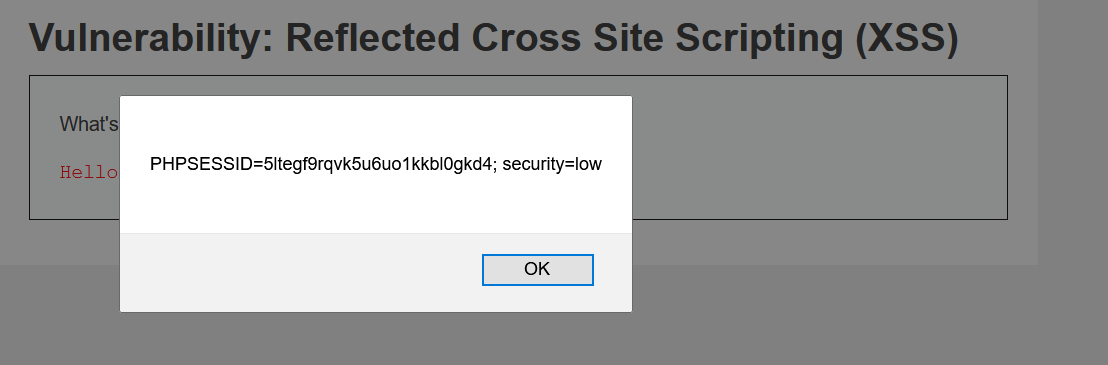
\includegraphics[width=\linewidth]{./imagenes/016_XSS_2.png}
    \caption{Ataque XXS.}  
    \label{fig:Ataque XXS.}
\end{figure}

Podemos distinguir tres tipos de ataques XSS:

\begin{itemize}
    \item \textbf{Reflejados:} Cuando el script malicioso esta presente en la petición HTTP.
    \item \textbf{Almacenados:} El script malicioso es almacenado en el servidor, en la base 
    de datos, en un fichero del sistema o cualquier otor objeto, y es visible cuando se muestra 
    la página en el navegador.
    \item \textbf{Basados en el DOM:} Técnicamente se consideraría reflejado. Ocurre cuando el script 
    malicioso incluye código html en la petición HTTP.
\end{itemize}

\subsection{A8:2017 - Deserialización insegura (Insecure Deserialization) }

Estos defectos ocurren cuando una aplicación recibe objetos serializados dañinos y estos objetos
pueden ser manipulados o borrados por el atacante para realizar ataques de repetición,
inyecciones o elevar sus privilegios de ejecución. En el peor de los casos, la deserialización
insegura puede conducir a la ejecución remota de código en el servidor. 

La serialización es el proceso de convertir un objeto en un formato de datos que se puede restaurar 
más tarde. Las personas a menudo serializan objetos para guardarlos en el almacenamiento o para enviarlos 
como parte de las comunicaciones. La deserialización es lo contrario de ese proceso que toma datos
estructurados de algún formato y los reconstruye en un objeto.

Hoy en día, el formato de datos más popular para serializar datos es JSON, no hace mucho el 
formato más común era XML.

Muchos lenguajes de programación ofrecen una capacidad nativa para serializar objetos. Estos formatos 
nativos suelen ofrecer más funciones que JSON o XML, incluida la personalización del proceso de 
serialización. Desafortunadamente, las características de estos mecanismos de deserialización 
nativos pueden reutilizarse para generar efectos maliciosos cuando se opera con datos que no son de confianza.

Se ha descubierto que los ataques de deserialización permiten ataques de denegación de servicio, control 
de acceso y ejecución remota de código. Los lenguajes de programación que se han conocido ataques de este 
tipo serian:

\begin{itemize}
    \item PHP
    \item Python
    \item Ruby
    \item Java
    \item C$\backslash$C++
\end{itemize}

Por ejemplo, este código Java aprovecha la serialización para codificar una tarea que detenga 
la aplicación durante 5 segundos:

\begin{listing}[h]
    \inputminted{java}{./Ficheros/Serialize.java}
    \caption{DTD example}
    \label{listing:2}
\end{listing}

Este código crea la tarea y la serializa generando el siguiente token:

\begin{verbatim}
    rO0ABXNyADFvcmcuZHVtbXkuaW5zZWN1cmUuZnJhbWV3b3JrLlZ1bG5lcmFibGVUYXNrSG9sZGVyAAAAAAAAAAICAANMABZyZXF1ZXN0ZWRFeGVjdXRpb25UaW1ldAAZTGphdmEvdGltZS9Mb2NhbERhdGVUaW1lO0wACnRhc2tBY3Rpb250ABJMamF2YS9sYW5nL1N0cmluZztMAAh0YXNrTmFtZXEAfgACeHBzcgANamF2YS50aW1lLlNlcpVdhLobIkiyDAAAeHB3DgUAAAflBgYSCgML+WfAeHQAB3NsZWVwIDV0AAZteVRhc2s=
\end{verbatim}

Dicho token al ser enviado en una petición al servidor provoca que la aplicación se detenga durante 5 segundos.

\subsection{A9:2017 - Uso de componentes con vulnerabilidades conocidas}

Los componentes como bibliotecas, frameworks y otros módulos se ejecutan con los mismos
privilegios que la aplicación. Si se explota un componente vulnerable, el ataque puede provocar
una pérdida de datos o tomar el control del servidor. Las aplicaciones y API que utilizan
componentes con vulnerabilidades conocidas pueden debilitar las defensas de las aplicaciones y
permitir diversos ataques e impactos.

\subsection{2.2.10. A10:2017 - Registro y monitoreo insuficientes}

El registro y monitoreo insuficiente, junto a la falta de respuesta ante incidentes permiten a los
atacantes mantener el ataque en el tiempo, pivotear a otros sistemas y manipular, extraer o
destruir datos. Los estudios muestran que el tiempo de detección de una brecha de seguridad es
mayor a 200 días, siendo típicamente detectado por terceros en lugar de por procesos internos. 



